\begin{figure*}[h]
        \begin{subfigure}{.66\columnwidth}
            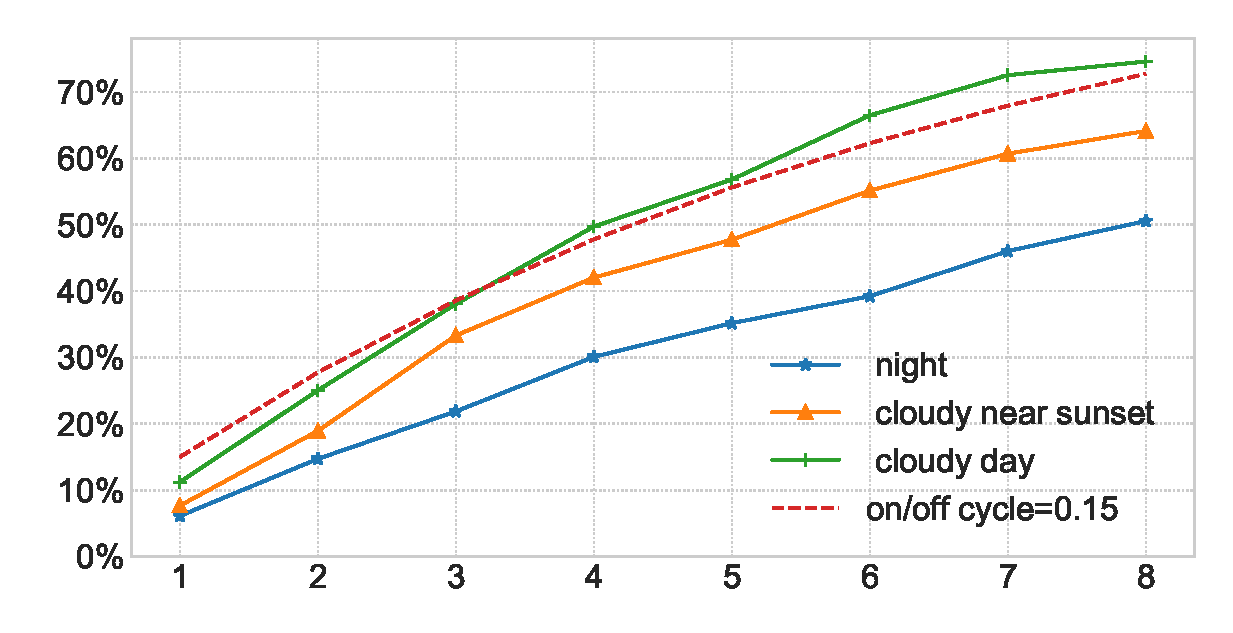
\includegraphics[width=\textwidth]{figures/sysAvailability}
                \caption{The \sys is powered by uncontrollable light sources---artificial light (night) and sunlight (day).}
            \label{fig:solarPwrCIS}
        \end{subfigure}\hfill
        \begin{subfigure}{.66\columnwidth}
            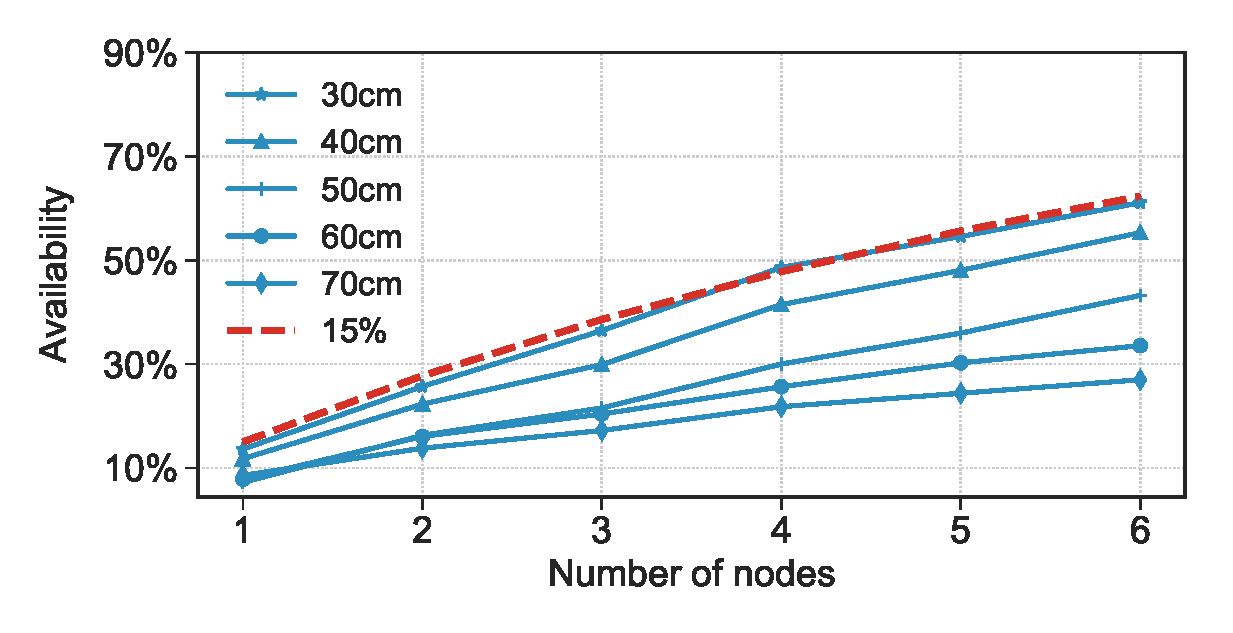
\includegraphics[width=\textwidth]{figures/rf_sysAvailability}
                \caption{The \sys is powered by an RF reader~\cite{r420_website} located 30-70\,cm aware from the RF tags (WISPs~\cite{smith_ubicomp_2006}).}
            \label{fig:rfPwrCIS}
        \end{subfigure}\hfill
        \begin{subfigure}{.66\columnwidth}
            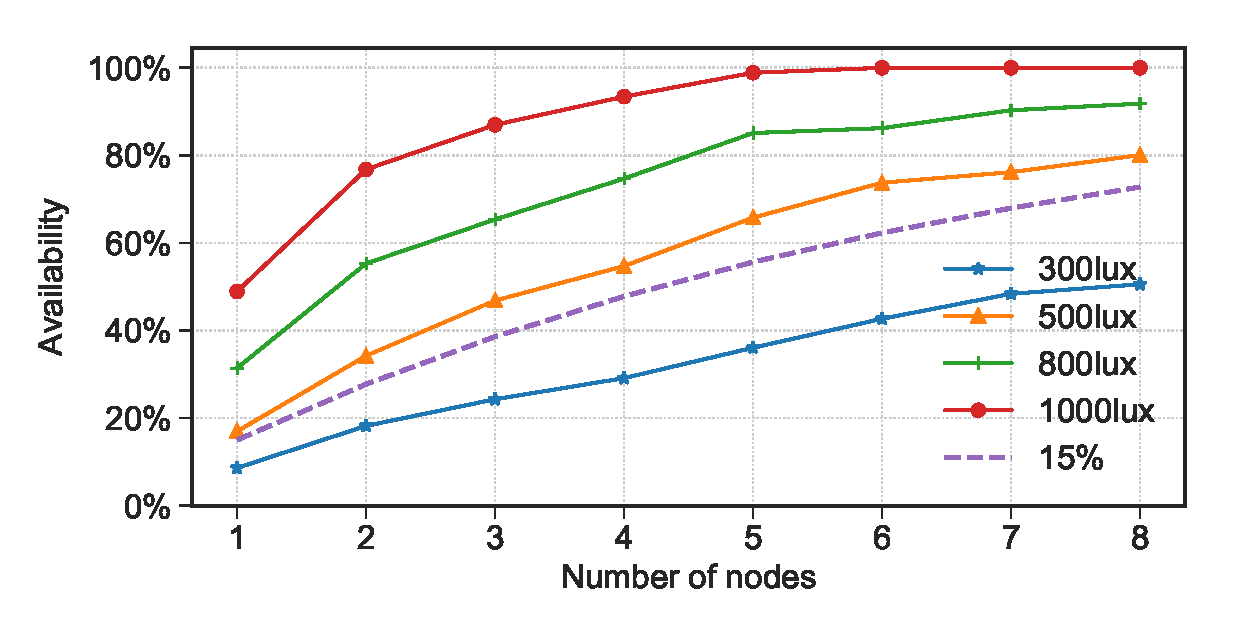
\includegraphics[width=\textwidth]{figures/sysAvailability_artificial-light}
                \caption{The \sys is powered by a controllable array of LEDs in a dark room. \vspace{1em}}
            \label{fig:rfPwrCIS}
        \end{subfigure}
        \caption{Measuring \fullsys availability for a differed number of intermittent nodes. Generally, adding a node increases the system availability. This increment, however, is proportional to the \sys off-time.}
        \label{fig:pwrCIS}
\end{figure*} 
To evaluate the performance of the \fullsys, we conducted several experiments in different energy conditions and with different event arrivals patterns. 
%
\subsection{Availability}
%%%%%%%%%% ToDo %%%%%%%%%%
% Experiment setup
In respective of the energy source (RF or light) we showed in Figure~\ref{fig:power_cycles} that the power cycles of a \sys's nodes are different, which leads to uniform distribution of their on-times, as we argued in Section~\ref{subSec:availability}. We captured the expected joined availability of these nodes in Equation~\ref{eq:cisModel}.  Here, we challenge our arguement and model by comparing the modeled availability of a \sys against the measured ones under different powering conditions and with different hardware. 
 
Figure~\ref{fig:pwrCIS} shows the availability of three \sys{}s when they are powered by different energy sources (sunlight, artificial light, and RF) and for a different number of intermittent nodes.
%%%%%%%%%% ToDo %%%%%%%%%%
% clarify that the RF and solar power nodes use different hardware.
The results clearly confirm our expectation: when the power cycles are slightly different, the on-times are uniformly distributed. And they validate our model (the dashed lines represent the modeled availability when the nodes duty cycle is 15\%).

\subsection{Sensing}
\subsubsection{Experiment setup}
\label{sec:experiment_setup}
% \paragraph{availability on a fine scale}
 % \todo{Because of the differences in intermittent nodes power cycles, their duty cycles are constantly shifting relative to each other ( Figure~\ref{fig:cisOntime}).  However, this study does zoom in on the \sys availability on short time scale and the effect of length of the differences between the nodes power cycles on the system short term availability. } 
%
\begin{table}[H]
\centering
\caption{Testing set}
\label{tab:words}
\begin{tabular}{lllll}
\hline
on    & off  & stop & clear & load   \\
go & pause & resume & edit  & cancel  \\  
\hline  
\end{tabular}
\end{table}
%
After validating our observation on different energy sources, we designed a testbed with controllable light intensity for clarity and results reproducible. To this end, we blocked uncontrollable light sources with a box of $60 \times 40$\,cm. On the box ceiling, we attached a light strip of 2.5\,m with 150 LEDs that can produce 15 different light intensities. On the bottom a \fullCIM of 8 intermittent nodes is placed (see Section~\ref{sec:hardware} for hardware description).

The events in our experiments are spoken words (Table~\ref{tab:words}). 
Short events (see events classification in Section~\ref{sec:event_classification}) are represented with individual words, while long burst events are represented with phrases of a few words.
We recorded different patterns of inter-event and inter-bust arriving time. We used a Bluetooth speaker~\cite{jbl} to replay a certain record. The data were collected using logic anaylyzer~\cite{saleae} and processed on a laptop running Ubuntu 16.04 LTS. 
%
\subsubsection{Events detection rate}
%
\begin{figure}[t!]
		\centering
	    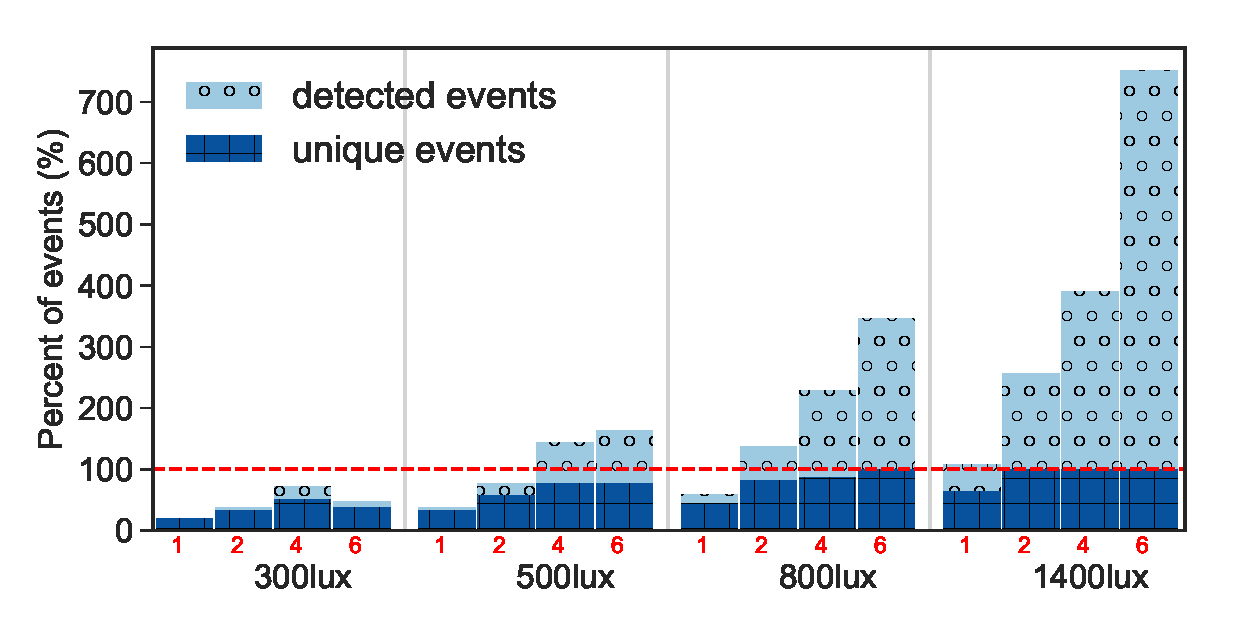
\includegraphics[width=\columnwidth]{figures/regular_events_capture_rate.eps}
		\caption{Duplicate and unique events captured by a \fullcim of eight solar-powered nodes. In general, we see that the number of captured events increases in tow case: when light intensity rises and when inter-event arrival time increases. 
         % In general, we see that when the light intensity increases, the number of detected and captured events rise too. Moreover, there is a positive correlation between the length of the inter-event arrival time and the detection and capture rates. 
         Red numbers indicate events arrival interval in seconds.
         }
    	\label{fig:events_detection_rate}
\end{figure} 
Here we experiment with the behavior of a \sys when events arrive individually or in bursts \emph{without} enabling  randomized response in favorable energy conditions. 
%
\begin{figure}[t]
    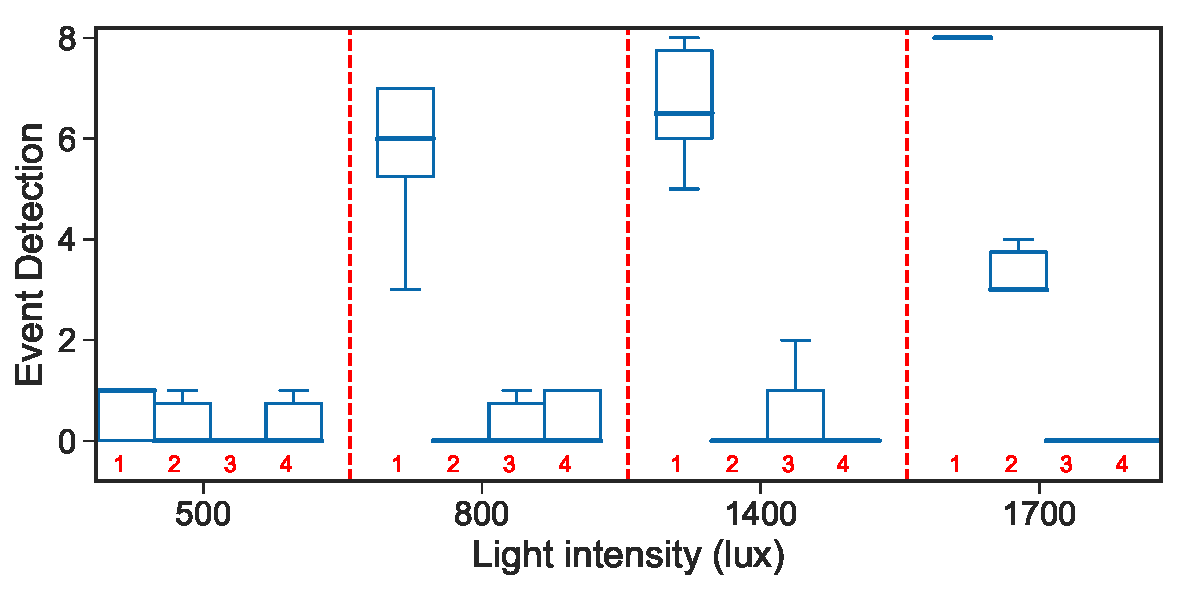
\includegraphics[width=\columnwidth]{figures/events_burst_problem}
	\caption{When capturing a burst of events without randomizing the response, the majority of the nodes react to the first event in the burst and power down shortly after, missing the rest of the burst. Red numbers indicate events index in a burst.}
    \label{fig:events_burst_problem}
\end{figure}
%
\paragraph{Individual events.}
\begin{figure}[t]
	\centering
     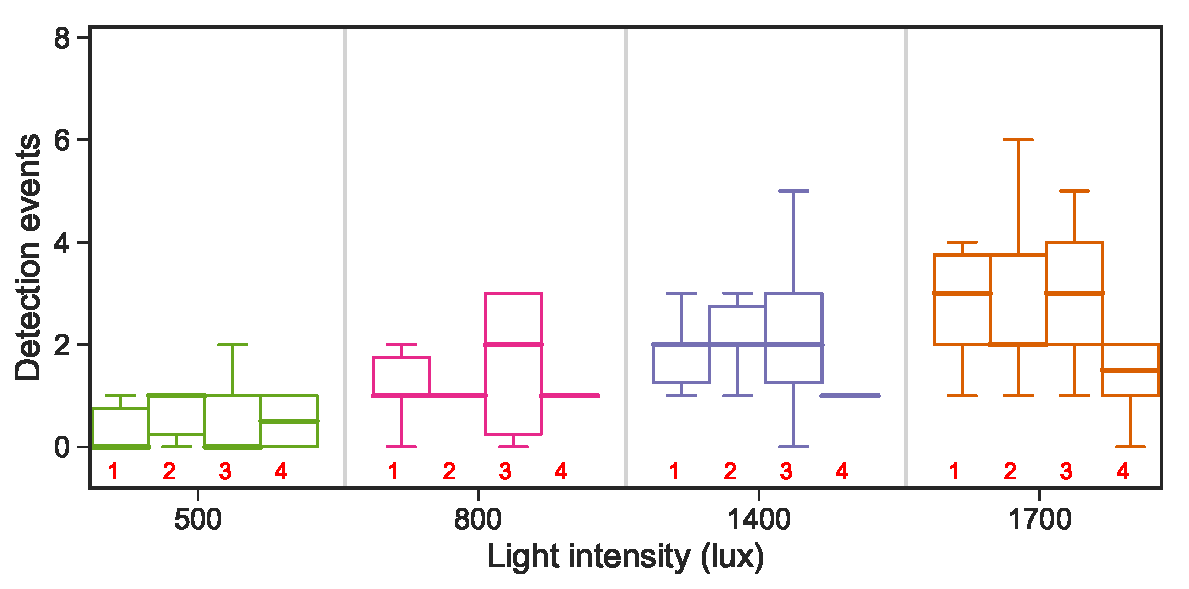
\includegraphics[width=\columnwidth]{figures/events_burst_rand}
    \caption{Response randomization enables a \sys to capture the entire burst of events with high capturing rates. It also reduces the number of duplicated events. Red numbers indicate events index in a burst.}
    \label{fig:events_burst_rand}
\end{figure}

Figure~\ref{fig:events_detection_rate} shows the percentages of capturing duplicate and unique events when light intensity varies from $\SI{300}{lux}$ to $\SI{1400}{lux}$ and the inter-event arrival time from $\SI{1}{sec}$ to $\SI{6}{sec}$. For each experimental trial 20 words were played, resulting in a total of 240 playbacks. 

We can clearly see a positive correlation between light intensity and the number of detected events. In particular, the number of duplicate detections rises dramatically when light intensity increases, \emph{demonstrating the overpowering problem} (Section~\ref{sec:power_state}). Moreover, increasing the inter-event arrival time also surges the number of duplicated events. The reason for this phenomenon is that when the time between events increases, the intermittent nodes get the chance to sleep longer in low-power mode, consuming less energy. Therefore, nodes' on-times expand, reducing their inherent randomization, which leads them to be in \textit{hibernating power state} (Section~\ref{it:hibernating}).  

% Indirectly, these results show how a \sys can achieve a much higher duty cycle than its individual intermittent nodes: Figure~\ref{fig:cis_nodes_dutyCycle} shows that with a light intensity of $\SI{800}{lux}$ an intermittent node is active with a duty cycle of 30\% while Figure~\ref{fig:events_detection_rate} shows that a \sys of 8 nodes captures 100\% of the unique events when the time between them is \SI{6}{s}. 

\paragraph{Bursty events.}
Figure~\ref{fig:events_burst_problem} shows the capturing behavior of a \sys when the events arrive in bursts. a burst of four events with one second between the individual event was fired every 20 seconds. Each burst was repeated 10 times and under four different light intensities. The nodes sleep in a low-power mode when they finish processing an event, waiting for the next one. 

In general, we observe that in favorable energy conditions (above $\SI{500}{lux}$) intermittent nodes react to the first event of a burst and power down shortly after missing the rest of the burst. These results confirm our theory about the side effect of the \textit{hibernating power state} of a \sys (Section~\ref{sec:power_state}). These results also demonstrate that the hibernating power problem happens on a wide range of power intensities, showing its significance. Next, we will show how randomizing the response can mitigate the problems generated when ambient energy exceeds the design point. 

\subsubsection{Events detection rate with randomization}
\begin{table}
	\centering
    $
    \begin{array}{llll}\hline
     \textbf{(lux,second)} & \textbf{(800,6)} & \textbf{(1400,4)} & \textbf{(1400,6)}\\\hline
    \textit{randomization}    & 205/432 &  236/675 & 223/493 \\
    \textit{no randomization} & 240/831 &  240/938 & 240/1802 \\\hline
    \end{array}
    $
    \caption{These results are presented in the following format \textit{unique/total} detected events. A \sys's node responds with a probability equals 65\% in the first two scenarios,\textbf{(800,6)} and \textbf{(1400,4)}, and 30\% for the last one.   
    We can see that Randomizing the response in this way reduces the number of duplicated events by 50\% while losing only 7\% of the unique events (if 7\% is two high, a higher responding probability can be used).}
    \label{tab:regular_rand}
\end{table}
% 
Here, we examine the effect of enabling artificial randomization on the \sys's response. 

\paragraph{Individual events.} 
Table~\ref{tab:regular_rand} compares the number of detected events when the \cim's response is randomized and not randomized.
When the randomization is enabled, nodes were responding to events with a probability of 65\% for the scenario of $\left(\SI{800}{lux}, \SI{6}{seconds}\right)$ and $\left(\SI{1400}{lux}, \SI{4}{seconds}\right)$, and for the highest energy level and the longest inter-event arrival time the responding probability was 30\%.

We see that randomizing the response reduces duplicated events by an average of $\approx$50\%, while only marginally lowers the number of the uniquely detected events. 

\paragraph{Bursty events.}
Figure~\ref{fig:events_burst_rand} shows how randomizing the \sys response spreads the nodes' awake times--as compared to Figure~\ref{fig:events_burst_problem}--and enables the \sys to capture the entire burst with a high probability, i.e., above 85\%. We also observe a positive impact of randomized response when the system is under-powered ($\SI{500}{lux}$).

To randomize during bursty events, a node reacts with a certain probability on a event. This probability is different for each event since the node become active after the last recharge. In order to spread the nodes over the events, the probabilities need to increase for subsequent events, since some nodes have reacted already on previous events, and therefore the number of nodes still available is smaller after each event.
A node reacts with a probability of 40\% on the first event, with 50\% on the second event, 70\% on the third event and 100\% on the fourth event.
%40 50 70 100


\subsection{Coalesced intermittent command recognizer word detection accuracy}
For evaluating the \fullcim accuracy, we used the word set in Table~\ref{tab:words}.
Each word was pronounced by a single speaker 20 times and recorded on a PC. One of these recordings was stored as a template on the \cim, while the remaining 19 were played back through a Bluetooth speaker~\cite{microphone} for testing.

The ratio between detected events and successfully recognized events per node is shown in Figure~\ref{fig:word_freq} and it averages out at  76.7\%. The difference between detection and capture is primarily caused by nodes that have insufficient buffered energy to finish recording.  

%
\begin{figure}
\centering
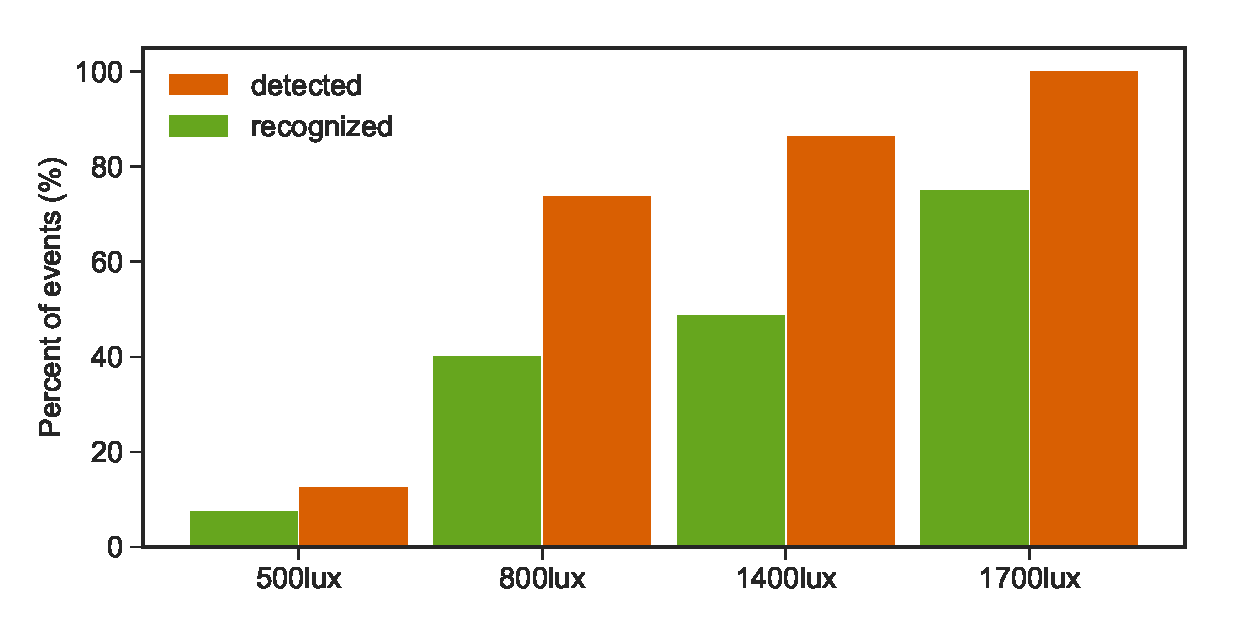
\includegraphics[width=\linewidth]{figures/detection_vs_recognition}
\caption{
% The percentage of successfully recognized words as compared to the detected ones.
Average number of successfully recognized words per node and average number of detected words per node, as percentages of the total number of played words. Words are relatively long events and therefore some of their recordings do not complete due to insufficient harvested energy.}
\label{fig:word_freq}
\end{figure}










































